\section{Technical overview}
\label{sec:poise__technical}

In this section, I first cover the general principles underlying, and the implementation of, POISE.
The basic operation of POISE is summarised in FIG, which is essentially a generalised version of the pure shift optimisations carried out in \cref{sec:pureshift__optimisation}.

\begin{figure}[htb]
    \centering
    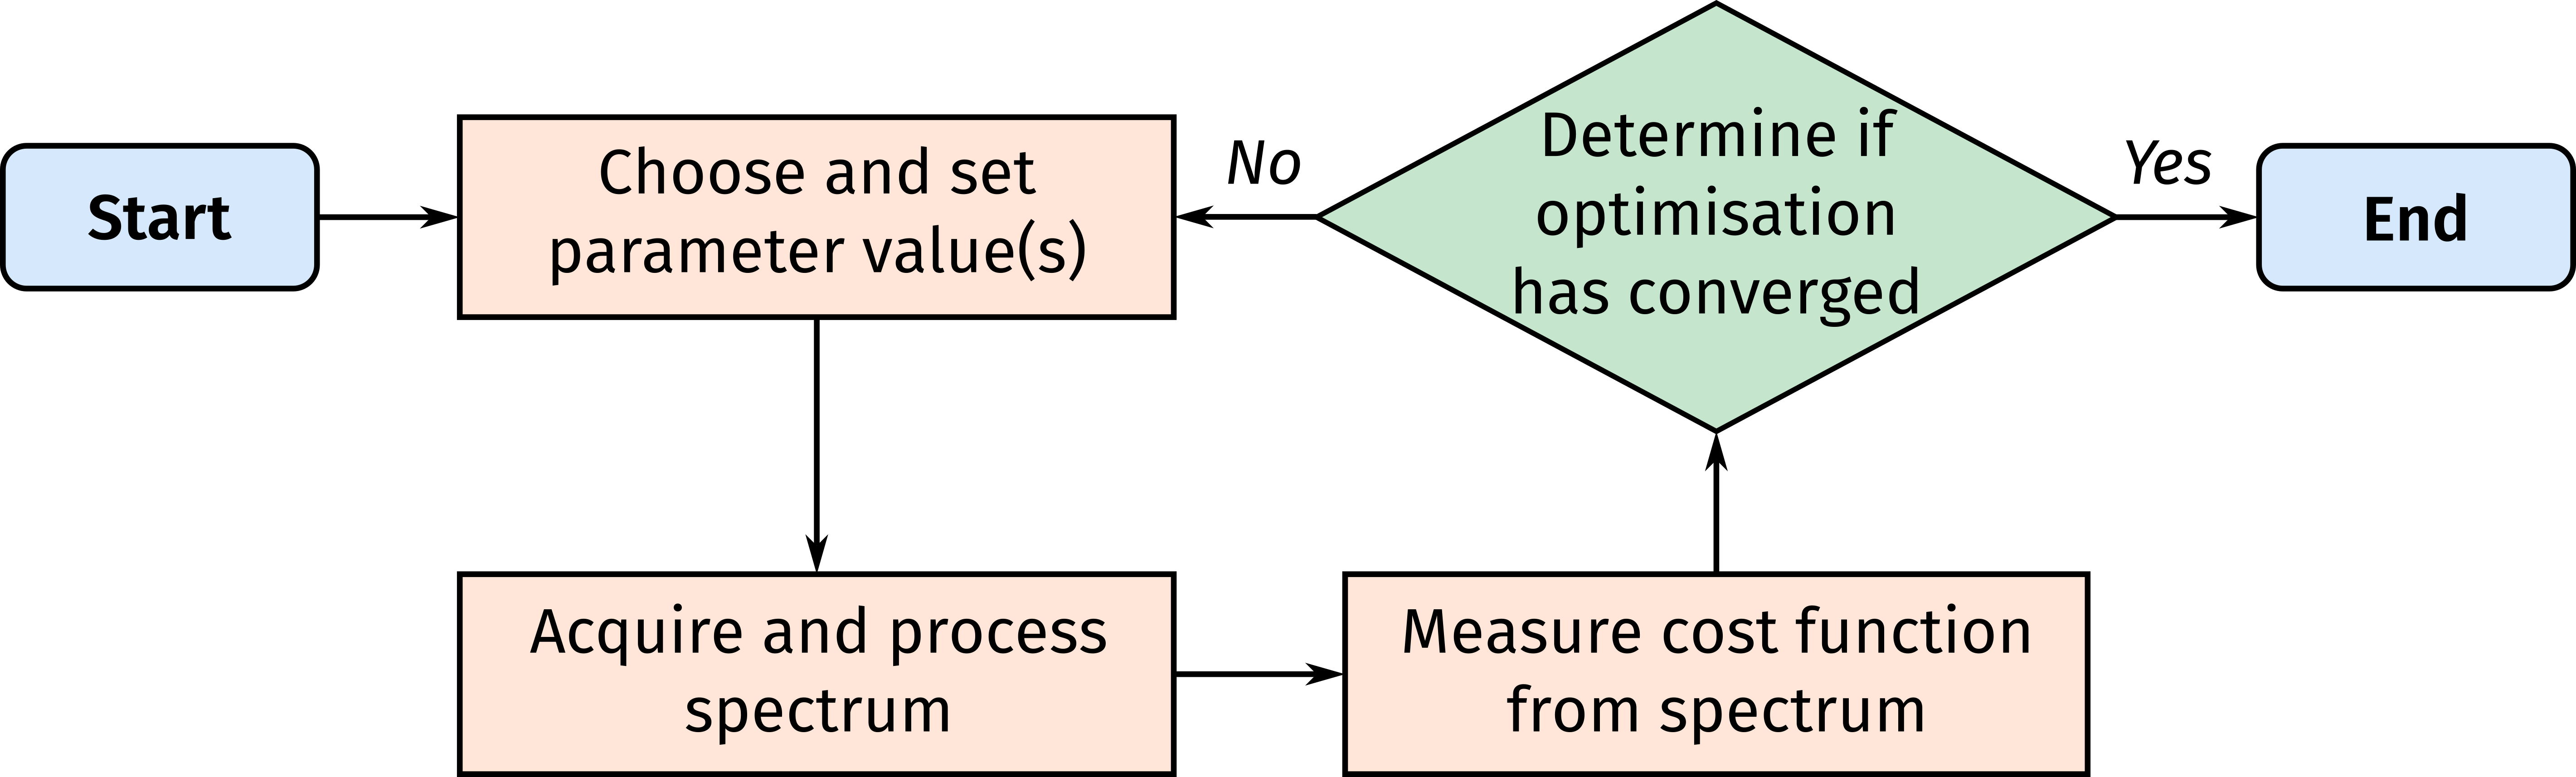
\includegraphics[draft=false]{poise/flowchart.png}
    \caption[Flowchart for POISE optimisations]{Flowchart depicting the main steps in a POISE optimisation.}
    \label{fig:poise_flowchart}
\end{figure}

Almost all aspects of this can be customised by the user, which I will now describe.
I make a distinction here between an optimisation \textit{routine}, as well as the \textit{settings} used to run these routines.
Routines consist of a series of predefined variables, such as the parameter(s) to be optimised: however, these may be optimised in different \textit{ways}, which is where the settings come in.
When discussing individual applications in \cref{sec:poise__applications}, I will make repeated reference to these components of an optimisation.

\subsection{Routines}
\label{subsec:poise__routines}

An \textit{optimisation routine}, as defined in POISE, consists of the following components:

\begin{enumerate}
    \item \textit{Name}

        This is an identifier used to refer to the entire routine, which is arbitrary, but should ideally be descriptive.

    \item \textit{Parameters}

        The parameters to be optimised.
        These are given as strings and directly correspond to TopSpin parameter names, for example, \texttt{P1} for a pulse width.

    \item \textit{Initial guess} (one per parameter)

        The point at which the optimisation is started.
        Naturally, this should represent the user's best guess at where the optimum lies.
        It is generally sensible to choose the unoptimised, `default' values for these.
        
    \item \textit{Lower} and \textit{upper bounds} (one each per parameter)

        Most parameters have a `chemically sensible' range, or alternatively, instrumental limits may sometimes restrict the range of parameter values which can be explored.

    \item \textit{Tolerances} (one per parameter)

        This loosely corresponds to the level of accuracy required for the optimisation.
        There is no point in setting this to be too small (i.e.\ requesting an overly accurate optimum), as the value of the cost function at two points too close together will likely differ only by noise.
        Furthermore, parameter values cannot be implemented with arbitrary precision on a spectrometer: the available resolution on this sets a lower bound for the tolerance (see \cref{subsec:poise__epsi} for a more concrete discussion of this).
        On the other hand, setting the tolerance to be too large may simply yield an imprecise and meaningless result.
        These conditions make it sound as if there is little room for error, but in practice getting the order of magnitude correct is usually enough (and the desired accuracy is also often reasonably clear from the context);

    \item \textit{AU programme}

        The AU programme defined here is used to acquire and process the spectrum.
        The user may leave this empty, in which case POISE automatically detects the dimensionality of the experiment and performs standard processing steps (Fourier transformation, window multiplication, phase correction, and baseline correction).
        However, this allows for almost infinite customisation of the actual spectral measurement: for example, the AU programme may call other scripts in TopSpin which create shaped pulses.

    \item \textit{Cost function}

        As before, this measures the `badness' of the spectrum thus recorded, and as before, the optimisation seeks to minimise this value.
        The cost function is written in Python 3: this design decision is considered later in \cref{subsec:poise__implementation}.
        Several cost functions which cover `typical' optimisation scenarios, such as maximising or minimising some signal intensity, come pre-installed with POISE, meaning that users do not necessarily need to write their own cost function if they are not familiar with Python.
\end{enumerate}

POISE allows users to create new routines interactively through a series of dialog boxes.
Alternatively, routines themselves can be created on-the-fly using the \texttt{poise --create} command: this is useful when some components are not known beforehand, such as if the optimum from a different optimisation is to be used as the initial point in a new one.
However, this is limited to single-parameter routines.

After being created, routines are stored in the human-readable JSON format: they can therefore be modified using any text editor.
Examples of these JSON files are presented in subsequent sections.

\subsection{Optimisation settings}
\label{subsec:poise__settings}

Once the user has defined a routine, it can then be run from the TopSpin command line using the command \texttt{poise ROUTINE\_NAME}.
However, the routine itself merely controls what parameters are being optimised: it does not specify what experiment is to be run (i.e.\ the pulse programme), nor any of the other parameters in the experiment.
These must be set by the user, and can most conveniently be stored in a TopSpin parameter set which can simply be loaded before starting the optimisation.
This flexibility means that the same \textit{type} of optimisation may be applied to different pulse sequences without having to create individual routines for each: for example, an experiment to optimise the NOE mixing time (as described in \cref{subsec:poise__noe}) can be run with different versions of the NOESY sequence depending on what is most appropriate.
Likewise, parameters such as the number of scans can be adjusted in order to run optimisations on samples with different concentrations.

Once the experiment parameters have been set up, there are a few more options which control how the optimisation is carried out:

\begin{itemize}
    \item the \texttt{-\phantom{}-maxfev} option allows the user to control the maximum number of FEs, or in other words, the maximum number of experiments run.
        If the optimisation has not converged after acquiring this many spectra, the best result so far is simply returned.
        This effectively allows the time spent on optimisation to be capped.

    \item the \texttt{-\phantom{}-quiet} option silences all output from the optimiser (the best parameters found are stored in the dataset itself after the optimisation ends, and can therefore be retrieved).
        This is useful when a POISE optimisation is to be run under automation.
        
    \item the \texttt{-\phantom{}-separate} option allows each FE to be run in a new experiment number, so that the optimisation trajectory can be analysed after its conclusion.

    \item perhaps most importantly, the \texttt{-\phantom{}-algorithm} option allows the user to choose one of three optimisation algorithms.
        I now describe these algorithms in greater detail.
\end{itemize}

\section{Implementation}
\label{sec:poise/implementation}

Blah.

Flowchart.

Python 3. Blah.

